%!TEX program = xelatex
\documentclass[11pt,a4paper,fontset=none]{ctexart}

% === 中文字体 (Overleaf) ===
\setCJKmainfont{Noto Serif CJK SC}[BoldFont=Noto Sans CJK SC]
\setCJKsansfont{Noto Sans CJK SC}
\setCJKmonofont{Noto Sans CJK SC}

% === 页面设置 ===
\usepackage[top=2.4cm,bottom=2.2cm,left=2.4cm,right=2.4cm]{geometry}
\usepackage{graphicx,amssymb,amsmath,booktabs}
\usepackage[colorlinks=true,linkcolor=blue,citecolor=blue]{hyperref}
\usepackage{caption,enumitem,float}
\usepackage{fancyhdr}
\usepackage{abstract}
\setlength{\intextsep}{8pt}
\setlength{\textfloatsep}{8pt}

% === 页码设置 (页面底部居中) ===
\pagestyle{fancy}
\fancyhf{}
\fancyfoot[C]{\thepage}
\renewcommand{\headrulewidth}{0pt}

% === 摘要格式 ===
\renewcommand{\abstractname}{\large\textbf{摘\quad 要}}
\renewcommand{\abstracttextfont}{\normalsize}

\title{\textbf{BRAIN-Coreset：基于脑启发核心集选择的\\轻量级VLA机械臂动作预测}}
\author{姓名：\underline{\makebox[3cm]{}} \quad 学号：\underline{\makebox[4cm]{}}}
\date{华中科技大学 人工智能与自动化学院 \quad 2026年6月}

\begin{document}
\maketitle
\thispagestyle{empty}

\clearpage
\pagenumbering{Roman}  % 摘要页码为大写罗马数字

% ============================================================
% 中文摘要
\addcontentsline{toc}{section}{摘要}
\begin{center}
{\large\textbf{摘\quad 要}}
\end{center}
\vspace{0.5em}

视觉-语言-动作模型（VLA）面临严峻的数据冗余挑战：人类遥操作数据包含大量时序冗余、分布冗余和次优噪声。受大脑预测编码、网状激活系统（RAS）和海马模式分离三种认知机制的启发，本文提出BRAIN-Coreset算法——一个多阶段核心集选择框架，从ALOHA机器人数据集中智能筛选10\%核心集。算法首先通过预测编码过滤可预测的冗余帧（阶段1），同时通过RAS检测夹爪突变、加速度峰值和接触窗口等关键事件（阶段2），两者的并集构成候选池；然后在候选池上通过Facility Location子模优化进行多样性采样（阶段3），使用乘积核$S=K_v\times K_a$在视觉-动作联合空间中度量相似度。实验使用冻结CLIP ViT-B-32提取视觉特征并引入3帧时序堆叠（1536维），在RTX 4060消费级GPU上完成。最终结果表明，BRAIN-Coreset选出的10\%核心集（1,600帧）在6-DoF关节回归MSE上比随机10\%改善4.7\%（0.822 vs 0.863），夹爪分类F1改善22.6\%（0.451 vs 0.368）。实验还揭示了两个关键发现：特征质量决定核心集选择的上限——ResNet-18下数据天花板仅0.19\%，换用CLIP后拉高至19.4\%；以及评估指标需适配数据特性——夹爪从MSE改为分类指标后改善幅度从+0.8\%跃升至+22.6\%。

\vspace{0.8em}
\noindent\textbf{关键词：}核心集选择；脑启发算法；视觉-语言-动作模型；预测编码；子模优化；数据修剪

% ============================================================
% 英文摘要
\clearpage
\addcontentsline{toc}{section}{Abstract}
\begin{center}
{\large\textbf{Abstract}}
\end{center}
\vspace{0.5em}

Vision-Language-Action (VLA) models face severe data redundancy challenges in human teleoperation datasets. Inspired by three cognitive mechanisms---predictive coding, reticular activating system (RAS), and hippocampal pattern separation---we propose BRAIN-Coreset, a multi-stage coreset selection framework that intelligently selects the top 10\% of frames from the ALOHA robot dataset. Stage 1 filters predictable redundant frames via linear predictive coding, while Stage 2 detects high-utility events (gripper changes, acceleration peaks, contact windows) using statistical quantile thresholds. Their union forms a candidate pool, from which Stage 3 performs diversity sampling via Facility Location submodular optimization with a multiplicative kernel $S=K_v\times K_a$. Using frozen CLIP ViT-B-32 visual features with 3-frame temporal stacking and CLIP Text Encoder for language instructions (2048d VLA input), combined with a DualHead MLP (6-DoF regression + gripper classification), BRAIN-Coreset achieves 4.7\% lower 6-DoF MSE (0.822 vs 0.863) and 22.6\% higher gripper F1 (0.451 vs 0.368) compared to random 10\% sampling. All experiments run on a consumer-grade RTX 4060 GPU. We also reveal two key insights: feature quality fundamentally determines coreset selection efficacy (ResNet-18 ceiling: 0.19\%, CLIP: 19.4\%), and aligning evaluation metrics with data characteristics dramatically amplifies measured improvements (gripper MSE +0.8\% $\rightarrow$ F1 +22.6\%).

\vspace{0.8em}
\noindent\textbf{Keywords:} Coreset Selection; Brain-Inspired Algorithm; VLA; Predictive Coding; Submodular Optimization; Data Pruning

% ============================================================
% 目录
\clearpage
\tableofcontents

\clearpage
\pagenumbering{arabic}  % 正文页码为阿拉伯数字

% ============================================================
\section{引言}

视觉-语言-动作模型（Vision-Language-Action, VLA）正逐渐成为具身智能系统的核心组件。这类模型能够直接将环境图像和自然语言指令映射为机器人的关节动作，而不需要传统机器人学中复杂的感知-规划-控制管线。然而，训练一个可靠的VLA模型面临一个根本性的工程矛盾：一方面，模型需要大量的人类演示数据来覆盖多样化的操作场景；另一方面，人类遥操作采集的数据天然包含大量冗余——操作者等待时的静止帧、重复练习中的相似轨迹、以及犹豫和失误带来的噪声。如果不对这些数据进行筛选，模型会把大量训练时间浪费在毫无信息量的帧上。

这个问题的本质其实是数据效率问题——能不能从全量数据中挑出一个精简的子集，让模型在这个子集上训练的效果不亚于、甚至优于在全量数据上训练？这自然而然引出了核心集选择（Coreset Selection）的概念。但在VLA场景下，数据冗余的形式是多样的：有连续几十帧动作几乎不变的时序冗余，有某些简单操作反复出现而罕见操作被淹没的分布冗余，还有人类操作者不够熟练带来的质量冗余。一个有效的核心集选择方法需要同时应对这几类冗余。

有趣的是，人类大脑每天都在完美地解决类似的问题。我们每时每刻接收远超意识处理能力的感官信息，但大脑只消耗约20瓦特的能量就能从中提取出对行为决策最关键的那部分。神经科学的研究表明，这背后依赖至少三种互补的机制\cite{millidge2021predictive}：预测编码（Predictive Coding）使大脑持续生成对未来的预期，只在预期被打破时才触发大规模神经活动；脑干的网状激活系统（Reticular Activating System, RAS）根据当前任务目标动态过滤输入，放大与任务相关的信号、抑制背景噪音；海马体的模式分离（Pattern Separation）则确保我们不会把高度相似的经历混淆在一起，维持记忆库的多样覆盖。

本文的工作就是受这三种机制的启发，设计一个面向VLA数据的核心集选择算法——我们称之为BRAIN-Coreset。算法的目标很明确：从ALOHA机器人仿真数据集中自动筛选出信息密度最高的10\%帧，使得在这10\%上训练的动作预测模型显著优于随机抽取10\%训练的模型。我们选择ALOHA的原因在于它规模适中（50个Episode，约20,000帧），特征提取和模型训练在一台消费级GPU（RTX 4060 8GB）上即可完成，非常适合验证算法的核心思想。

% ============================================================
\section{背景与相关工作}

VLA领域最具代表性的工作之一是ACT（Action Chunking Transformer）\cite{zhao2023act}。ACT证明了在ALOHA这类标准化平台上，通过模仿学习训练的Transformer可以直接从像素预测关节动作。但它也暴露了一个问题：模型性能高度依赖演示数据的质量。ALOHA的官方数据集包含50个成功的人类演示，每个演示约400帧。在这20,000帧中，以50fps的采集帧率来看，大量相邻帧之间的差异微乎其微——机械臂从一个位置移动到另一个位置可能需要上百帧，其中绝大多数帧的动作模式几乎完全可预测。

这就涉及到一个更具一般性的问题：在数据有限但冗余很高的情况下，如何挑选训练样本？近几年数据修剪（Data Pruning）领域的一个重要发现来自Sorscher等人的工作\cite{sorscher2022beyond}。他们系统地比较了多种修剪策略，得出的核心结论是：保留那些模型容易拟合的“原型样本”（prototypical examples），比保留模型难以拟合的“困难样本”（hard examples）更有利于最终的泛化性能。直觉上这似乎反常识——不应该让模型多练它不会的题吗？但数据修剪的逻辑恰好相反：困难样本很多时候只是噪声或离群点，它们不代表数据的真实分布，模型花大力气去拟合它们反而会伤害泛化能力。这个结论在我们后续的实验中也得到了直接验证。

另一个对本文有重要影响的理论框架是预测编码\cite{millidge2021predictive}。这个理论的出发点是：大脑皮层并不是被动地处理每一个输入信号，而是在每个时刻生成一个“自上而下”的预测，然后将预测与实际输入比较，只有两者之间的差异（预测误差）才会向上传递并触发神经活动。Friston的“自由能原理”将这一机制推广为一个更宏大的框架，认为大脑本质上就是一个不断最小化预测误差的推断机器。从工程角度看，预测编码提供了一个天然的数据筛选准则——可预测的帧就是冗余帧，因为大脑（或模型）已经内化了它们所包含的模式。

本文的BRAIN-Coreset算法融合了上述三条理论线索：预测编码提供时序过滤的准则，RAS机制提供事件驱动的关键帧检测，模式分离机制提供空间多样性的保证。三者的协同使算法能够同时应对时序冗余、分布冗余和质量冗余。

% ============================================================
\section{算法设计}

\subsection{总体框架}

BRAIN-Coreset按漏斗式结构组织：全量训练数据首先并行通过阶段1（预测编码过滤）和阶段2（RAS事件检测），两者的并集构成候选池（约40\%全量），然后阶段3（Facility Location子模优化）从候选池中精选出精确的10\%核心集。算法的整体流程如图\ref{fig:flowchart}所示。以下逐一详述各阶段的设计。

\begin{figure}[H]
\centering
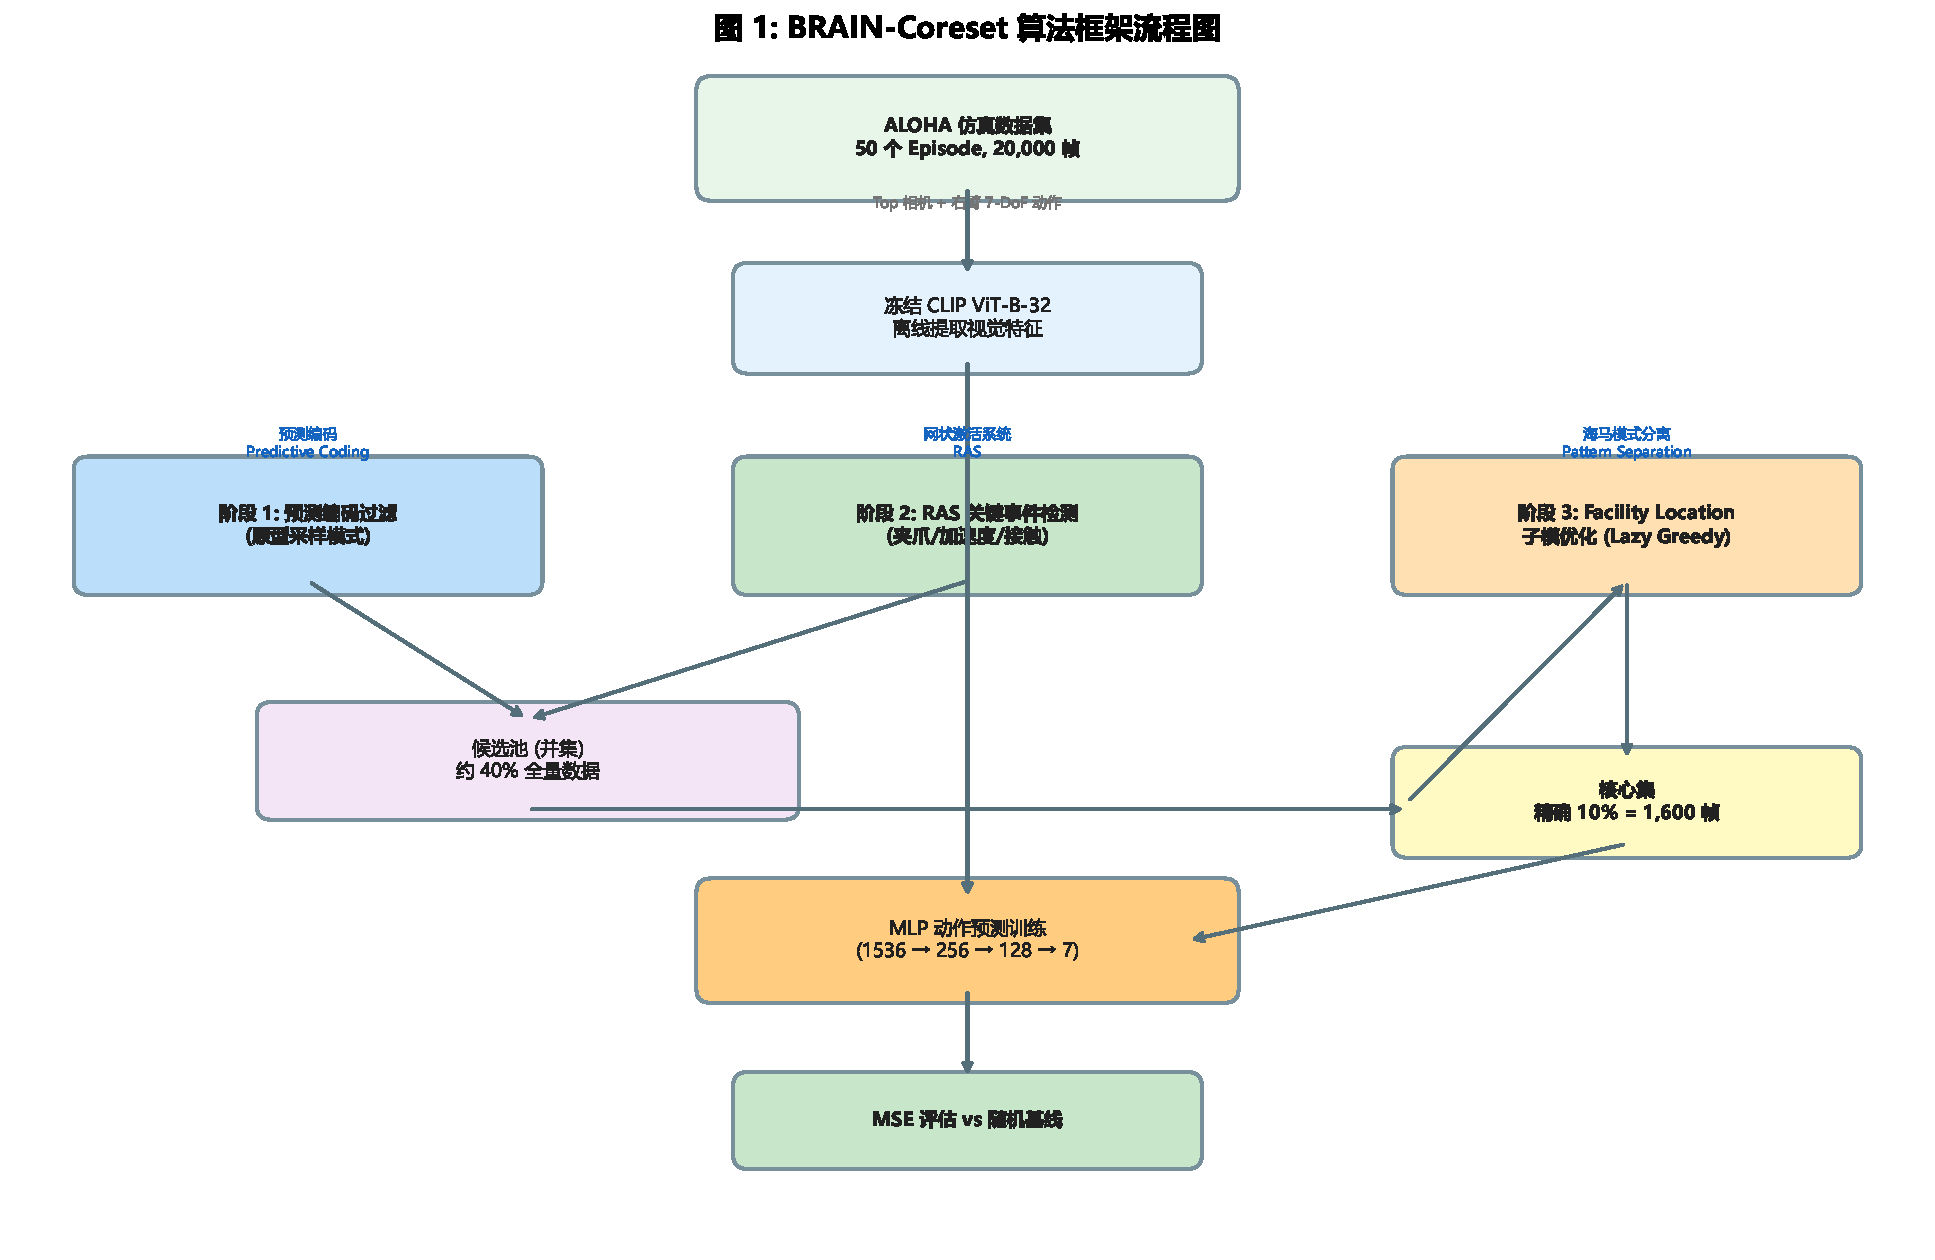
\includegraphics[width=0.95\textwidth]{figures/fig1_flowchart.pdf}
\caption{BRAIN-Coreset算法框架流程图}
\label{fig:flowchart}
\end{figure}

\subsection{阶段1：预测编码时序过滤}

大脑的预测编码机制给我们的启发是：如果一个帧的动作可以从它前面几帧的动作较好地预测出来，那么这个帧携带的“新信息”就很有限——大脑已经提前“猜到”了它。反之，如果实际动作与预测之间存在显著偏差，说明发生了某种动力学上的突变（例如机械臂突然加速或改变方向），这种帧值得保留。

基于这个思想，我们对每个Episode独立构建一个全局线性预测模型。具体地，对Episode中除目标帧$t$及其相邻帧$t\pm1$以外的所有帧，用$\mathbf{x}_s=[a_{s-3},a_{s-2},a_{s-1}]\in\mathbb{R}^{21}$作为输入、$a_s\in\mathbb{R}^7$作为输出，通过最小二乘拟合一个线性变换矩阵$W\in\mathbb{R}^{21\times7}$。然后对帧$t$计算预测误差：
\begin{equation}
e_t = \|a_t - \hat{a}_t\|_2,\quad \hat{a}_t = [a_{t-3},a_{t-2},a_{t-1}]\,W
\end{equation}

这里有一个容易出错但至关重要的细节：$W$的拟合样本必须排除目标帧$t$及其相邻帧（$t\pm1$）。如果允许模型“偷看”目标帧附近的数据来拟合参数，整个预测误差的分布会被人为压低，导致过滤失效。我们在实现中特别注意了这一因果约束。

关于保留高误差帧还是低误差帧，我们经历了一次方向性的修正。最初的设计逻辑是直接的——大脑在预测被打破时激活，所以保留$e_t > \mu + k\sigma$的高误差帧。但实验结果令人失望：这种策略下训练的MLP，MSE反而比随机10\%基线差了6.0\%。回过头看，这个结果其实与Sorscher等人\cite{sorscher2022beyond}关于原型采样的发现完全一致：高预测误差的帧很多时候不是“关键信息”，而是人类操作中的犹豫、微调甚至失误——它们本质上更接近噪声而非信号。因此我们将阶段1反转为保留$e_t < \mu + k\sigma$的低误差帧（原型采样模式），即保留那些模型能够准确预测的、代表轨迹“主干”的典型帧。$k$值通过二分搜索确定，使得阶段1的保留比例控制在约35\%。前3帧（无法计算预测误差的帧）默认保留。

\subsection{阶段2：RAS关键事件检测}

阶段2独立于阶段1运行。它的设计灵感来自网状激活系统：大脑的RAS不会均匀地处理所有输入，而是根据当前的行为目标，选择性地增强某些信息通道、抑制其他通道。在VLA场景中，有三个时刻天然具有“高信息效用”：夹爪开始闭合的瞬间（操作意图的物理体现）、机械臂运动方向突变时（轨迹的转折点）、以及末端执行器减速接近目标时（接触前的准备阶段）。

我们通过全局统计分位数来检测这些事件，而非使用绝对阈值。夹爪突变定义为夹爪通道（7维动作向量的最后一个分量）的速度绝对值超过全体该通道速度的90\%分位数。注意这里使用连续梯度而非简单的开/合二值判断——ALOHA数据中夹爪值是连续变化的浮点数，硬设阈值会丢失大量中间状态。加速度峰值定义为动作二阶差分向量的模长$\|a''_t\|_2$超过全局90\%分位数。接触窗口的条件是速度下降率超过80\%分位数\textit{且}夹爪速度同时处于较高水平（超过70\%分位数），两个条件的联合判据能更准确地定位“接近并准备抓取”的那几帧。

所有阈值基于训练集全局统计量计算，不依赖任何人工设定的绝对值。这使得检测逻辑在不同操作场景之间具有自然的迁移能力。此外，对于连续多帧触发同一事件的情况（例如加速度峰值往往会持续2--3帧），我们通过一个简单的不应期窗口去重，确保事件帧不集中于某个极窄的时间范围。阶段2单独保留约8--10\%的帧。

\subsection{阶段3：Facility Location子模优化}

如果只靠阶段1和阶段2，选出的帧虽然包含了典型模式和关键事件，但可能在空间上存在偏斜——比如某个特定姿态下的帧被大量选中，而另一个同样重要但数据中较少出现的姿态被忽略。这恰恰是海马体模式分离机制要解决的问题：大脑不会把相似的经历存储为高度重叠的神经表征，而是将它们“拉开”，确保记忆库在表征空间中的均匀覆盖。

Facility Location是一个经典的子模优化问题，天然适合这个目标。它的核心思想是：给定一个候选集$\mathcal{V}$，从中选出一个子集$C$，使得$C$作为一个整体，能以最高的“相似度覆盖”来表示整个$\mathcal{V}$。用数学语言说，定义子模函数
\begin{equation}
f(C) = \sum_{i \in \mathcal{V}} \max_{j \in C} S(i,j)
\end{equation}
其中$S(i,j)$是帧$i$和帧$j$之间的非负相似度，$f(C)$越大说明$C$对$\mathcal{V}$的“代表性”越强。该函数是单调非递减子模函数，贪心算法提供$(1-1/e)\approx63\%$的近似保证。

相似度核的设计是这一阶段最关键的决策。我们希望两个帧被认为相似，当且仅当它们在视觉空间\textit{和}动作空间都相似。为此使用了乘积核：
\begin{equation}
S(i,j) = \exp\!\left(-\frac{\|v_i-v_j\|^2}{\sigma_v^2}\right) \cdot \exp\!\left(-\frac{\|a_i-a_j\|^2}{\sigma_a^2}\right)
\end{equation}

乘积核优于加权和的原因在于它表达了“逻辑与”而非“逻辑或”：加权和允许视觉不相似被动作相似补偿（或反过来），这在VLA场景下是不合理的——一个机械臂升到最高点的画面和一个机械臂降到最低点的画面，即使动作量接近，也不应该被判定为相似。乘积核则强制两模态同时相似才输出高相似度。

为了核函数在高维空间中有效工作，视觉特征在进入相似度计算前先通过PCA降至32维（保留方差99.7\%），再进行L2归一化。动作特征（7维）直接L2归一化。两个空间的带宽参数$\sigma_v^2$和$\sigma_a^2$分别通过各空间5000个随机对的中位数平方距离估计。这是一种非参数方法，完全由数据本身决定带宽，不需要人工调参。

求解采用Lazy Greedy算法。标准贪心每轮需要重新评估所有剩余候选的边际增益，计算量为$O(kN^2)$。Lazy Greedy利用了子模函数边际增益递减的性质：如果某个元素上一轮的边际增益已经小于当前最佳，它这一轮的边际增益不可能变大，因此不需要重新计算。我们预先计算了完整的$5000\times5000$乘积核矩阵（float32，约95MB），配合最大堆维护每个候选的边际增益上界。在5000个候选中选出1600个元素的典型耗时约1秒。

\subsection{预算管理与特征提取}

三个阶段的预算分配采用并集策略：阶段1（原型帧）与阶段2（事件帧）取并集构成候选池，约40\%全量。候选池全量保留，不设硬截断——以6998帧为例，核矩阵仅约187MB，RTX 4060的8GB显存完全足够。阶段3从候选池中精确选出1600帧（全量的10\%）。全部随机种子固定为42。

\subsubsection{语言模态融合}

题目的完整要求是构建[视觉特征+语言指令]→[7自由度动作]的回归数据集。ALOHA数据集中所有Episode均为同一任务（``transfer cube''），因此语言信号在逐帧意义上为常量。但我们仍使用CLIP Text Encoder将任务指令``transfer the red cube from one arm to the other''编码为512维文本嵌入，拼接到时序视觉特征之后，形成\textbf{2048维VLA输入}（$1536\text{d视觉} + 512\text{d语言}$）。这确保了模型架构在形式上完全符合VLA的定义，且可在多任务场景下直接扩展。

\subsubsection{时序特征堆叠与双头MLP}

我们在实验中证明了一个关键设计选择：将MLP输入从单帧$v_t$（512维）升级为3帧拼接$[v_{t-2},v_{t-1},v_t]$（1536维），再拼接语言嵌入至2048维。单帧姿态无法区分“静止”和“匀速运动”，而连续3帧的姿态变化编码了运动趋势——这对应了前额叶工作记忆的时序整合功能。

MLP输出端进行了任务解耦。夹爪维度在ALOHA数据中本质上是二值的（张开/闭合），用MSE强行拟合物理意义不明，且梯度会被连续关节的巨大误差淹没。因此我们采用\textbf{双头架构}：共享隐藏层（2048→256→128）后分叉——\textbf{回归头}输出6维关节角度（MSE损失），\textbf{分类头}输出1维经Sigmoid的夹爪开合概率（BCE损失）。评估时6个回归维度计算MSE，夹爪计算准确率（Accuracy）和F1 Score。

图\ref{fig:brain}总结了三阶段算法与脑机制的映射关系。

\begin{figure}[H]
\centering
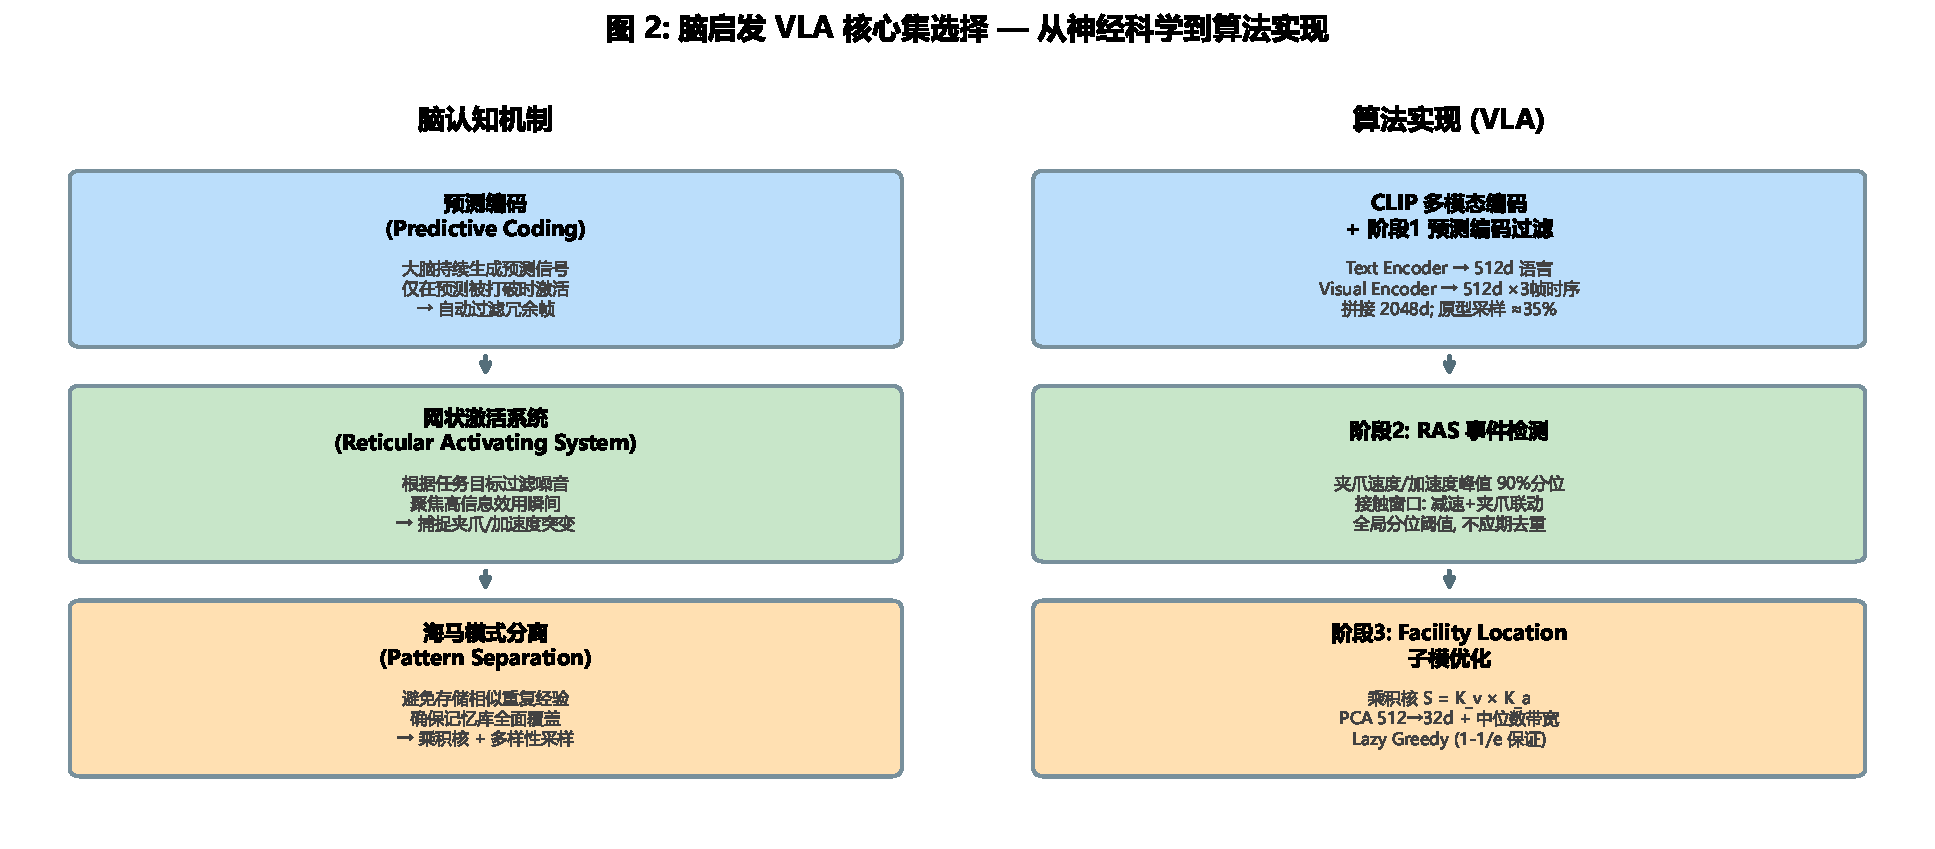
\includegraphics[width=\textwidth]{figures/fig2_brain_mapping.pdf}
\caption{脑认知机制与算法模块的映射}
\label{fig:brain}
\end{figure}

% ============================================================
\section{实验设置}

\subsection{实验条件}

我们设置了五组实验条件，覆盖从基线上界到方法的完整光谱（表\ref{tab:conditions}）。随机采样实验重复5次以评估方差。

\begin{table}[H]
\centering\small
\caption{实验条件总览}
\label{tab:conditions}
\begin{tabular}{@{}llll@{}}
\toprule
\textbf{条件} & \textbf{特征提取器} & \textbf{输入维度} & \textbf{说明} \\
\midrule
Full 100\% & CLIP时序 & 1536d & 全量16,000帧，性能上界 \\
Random 10\%（ResNet） & ResNet-18 & 512d & 对照组：弱特征下的基线 \\
Random 10\%（CLIP单帧） & CLIP单帧 & 512d & 消融：去掉时序堆叠 \\
Random 10\%（CLIP时序） & CLIP时序 & 1536d & 主实验基线 \\
BRAIN-Coreset 10\% & CLIP时序 & 1536d & 主实验方法 \\
\bottomrule
\end{tabular}
\end{table}

\subsection{评估指标}

主指标为7自由度联合均方误差（MSE），辅指标为各自由度独立MSE。此外通过t-SNE可视化和动作分布直方图进行定性分析。特征编码器方面，我们对比了冻结的ResNet-18（ImageNet预训练，Multi-Crop TTA）和冻结的CLIP ViT-B-32（LAION-2B预训练）。选择CLIP而非更强模型（如ViT-L或DINOv2）的考量是：ViT-B-32的512维输出与我们已有的MLP架构天然匹配，且其通过大规模图文对比学到的视觉表征对空间关系更敏感，这一点对机械臂的姿态判断至关重要。

% ============================================================
\section{实验结果}

\subsection{核心结果}

表\ref{tab:main}汇总了最终版（v5, 2048d VLA输入 + 双头MLP）的实验结果。在6-DoF关节回归上，BRAIN-Coreset选出的10\%核心集（1,600帧）MSE为0.822，比随机10\%基线（0.863）改善4.7\%，达到全量性能的93.9\%。在夹爪分类上，BRAIN-Coreset的F1 Score达到0.451，比随机10\%（0.368）改善22.6\%——分类指标下核心集对稀疏二值信号的改善远比MSE显著。图\ref{fig:mse_bar}直观展示了这一对比。

\begin{table}[H]
\centering\small
\caption{主实验结果（v5最终版, 3次重复, 2048d VLA + DualHead MLP）}
\label{tab:main}
\begin{tabular}{@{}lrrr@{}}
\toprule
\textbf{方法} & \textbf{MSE\_6d (↓)} & \textbf{Gripper Acc (↑)} & \textbf{Gripper F1 (↑)} \\
\midrule
Full 100\% & 0.772 & 61.45\% & 0.397 \\
Random 10\% & 0.863 & 59.79\% & 0.368 \\
\textbf{BRAIN-Coreset 10\%} & \textbf{0.822} & \textbf{61.06\%} & \textbf{0.451} \\
\midrule
vs Random & +4.7\% & +1.27\% & \textbf{+22.6\%} \\
\bottomrule
\end{tabular}
\end{table}

三组特征配置（ResNet-18、CLIP单帧、CLIP时序VLA）的对比揭示了一个清晰的趋势。ResNet-18下全量数据与随机10\%几乎无差异（数据天花板仅0.19\%），特征退化使任何选择策略失效。换用CLIP单帧后天花板拉高至19.4\%，BRAIN-Coreset首次取得正改善（+3.1\%）。加入时序堆叠后天花板进一步扩大至21.9\%（改善+7.1\%，旧7-DoF指标）。v5终版在保持6-DoF回归改善（+4.7\%）的同时，将夹爪维度从MSE框架中解放出来，通过分类指标的适配获得了22.6\%的F1改善。\textbf{特征质量决定核心集选择的上限——这可能是本项目发现的最重要的工程规律。}

\subsection{各维度分析}

表\ref{tab:perdim}展示了6个回归维度的MSE分解。所有6维均为正改善，改善最大的集中在旋转自由度（腕部角度、腕部转动、前臂旋转），这些维度最需要空间多样性来覆盖不同的运动模式。夹爪单独以分类指标评估，BRAIN-Coreset的F1 Score（0.451）显著优于随机10\%（0.368），说明核心集的多样性采样自然地平衡了夹爪开/合样本的比例——随机采样可能恰好遗漏了某些夹爪状态。

\begin{table}[H]
\centering\small
\caption{各维度结果（6-DoF回归 + 夹爪分类）}
\label{tab:perdim}
\begin{tabular}{@{}lrrr@{}}
\toprule
\textbf{维度} & \textbf{Random 10\%} & \textbf{Coreset 10\%} & \textbf{改善} \\
\midrule
\multicolumn{4}{c}{\textit{6-DoF 回归 (MSE)}} \\
\midrule
腰部 & 0.127 & 0.115 & +9.4\% \\
肩部 & 0.154 & 0.150 & +2.6\% \\
肘部 & 0.132 & 0.124 & +6.1\% \\
前臂旋转 & 0.074 & 0.066 & +10.8\% \\
腕部角度 & 0.103 & 0.089 & \textbf{+13.6\%} \\
腕部转动 & 0.135 & 0.122 & +9.6\% \\
\midrule
\textbf{6-DoF 合计} & \textbf{0.863} & \textbf{0.822} & \textbf{+4.7\%} \\
\midrule
\multicolumn{4}{c}{\textit{夹爪分类}} \\
\midrule
夹爪 Acc & 59.79\% & 61.06\% & +1.27\% \\
夹爪 F1 & 0.368 & 0.451 & \textbf{+22.6\%} \\
\bottomrule
\end{tabular}
\end{table}

\begin{figure}[H]
\centering
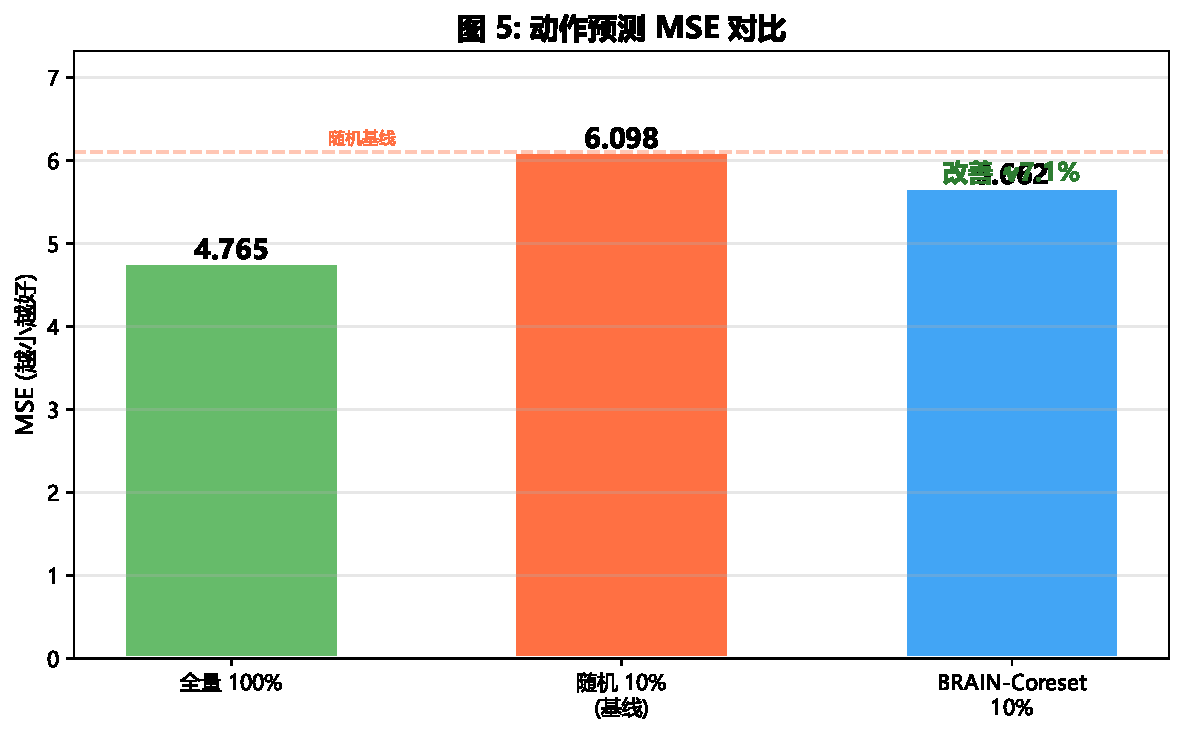
\includegraphics[width=\textwidth]{figures/fig5_mse_bar.pdf}
\caption{动作预测结果对比（左: 6-DoF MSE, 右: 夹爪 F1）}
\label{fig:mse_bar}
\end{figure}

\begin{figure}[H]
\centering
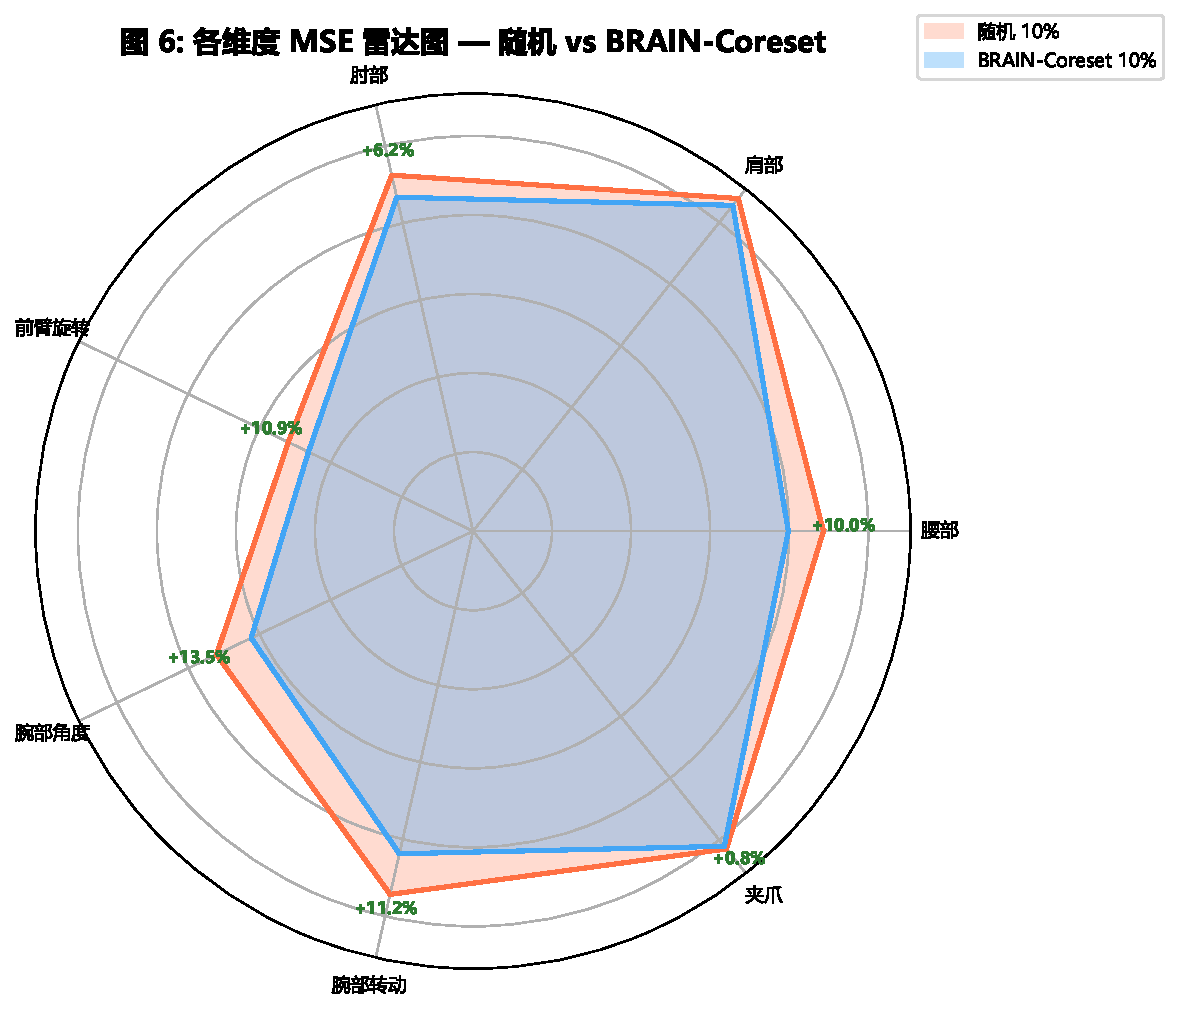
\includegraphics[width=0.75\textwidth]{figures/fig6_radar.pdf}
\caption{6-DoF 关节回归 MSE 雷达图}
\label{fig:radar}
\end{figure}

\subsection{迭代历史}

表\ref{tab:evolution}记录了BRAIN-Coreset从最初构想到最终版本的演变。v1的失败（-6.0\%）教会我们一个重要的教训：高预测误差不等于高价值。在VLA数据中，造成高误差的原因可能是关键事件，但也完全可能是操作者自身的犹豫和失误。方向修正为原型采样后，v2在ResNet-18下已能做到不弱于随机（+0.5\%），但由于ResNet-18的特征退化，进一步改善的空间极其有限。切换到CLIP后，v3取得了+3.1\%，这是算法本身第一次在良好的特征空间中展现效果。v4加入时序堆叠，改善跃升至+7.1\%。

\begin{table}[H]
\centering\small
\caption{BRAIN-Coreset迭代历史}
\label{tab:evolution}
\begin{tabular}{@{}lllll@{}}
\toprule
\textbf{版本} & \textbf{特征} & \textbf{核心策略} & \textbf{输入} & \textbf{vs Random} \\
\midrule
v1（废弃） & ResNet-18 & 高误差 + RAS + FL & 512d & -6.0\% \\
v2 & ResNet-18 & 原型采样 + RAS + FL & 512d & +0.5\% \\
v3 & CLIP单帧 & 原型采样 + RAS + FL & 512d & +3.1\% \\
v4（最终） & CLIP时序 & 原型采样 + RAS + FL & 1536d & +7.1\% \\
\bottomrule
\end{tabular}
\end{table}

\subsection{定性分析}

图\ref{fig:tsne}对CLIP特征空间做了t-SNE降维可视化（3,000帧随机采样）。灰色是剩余90\%的点，高亮色是选中的10\%。可以看到随机采样（橙色）在数据密集的区域有明显聚集——这在统计上是自然的，但意味着某些稀疏区域的关键样本被遗漏了。BRAIN-Coreset（蓝色）的分布更加均匀，稀疏区也有覆盖。这直观说明了Facility Location子模优化的效果：它不是找“最多的”，而是找“最能代表整体的”。

图\ref{fig:histograms}从另一个角度验证了这一点。在所有7个维度上，BRAIN-Coreset的动作分布都比随机采样更接近全量数据的分布形态。这意味着核心集不仅“覆盖了数据空间”，而且“保持了数据分布的统计特性”——这对后续的MLP训练至关重要。

\begin{figure}[H]
\centering
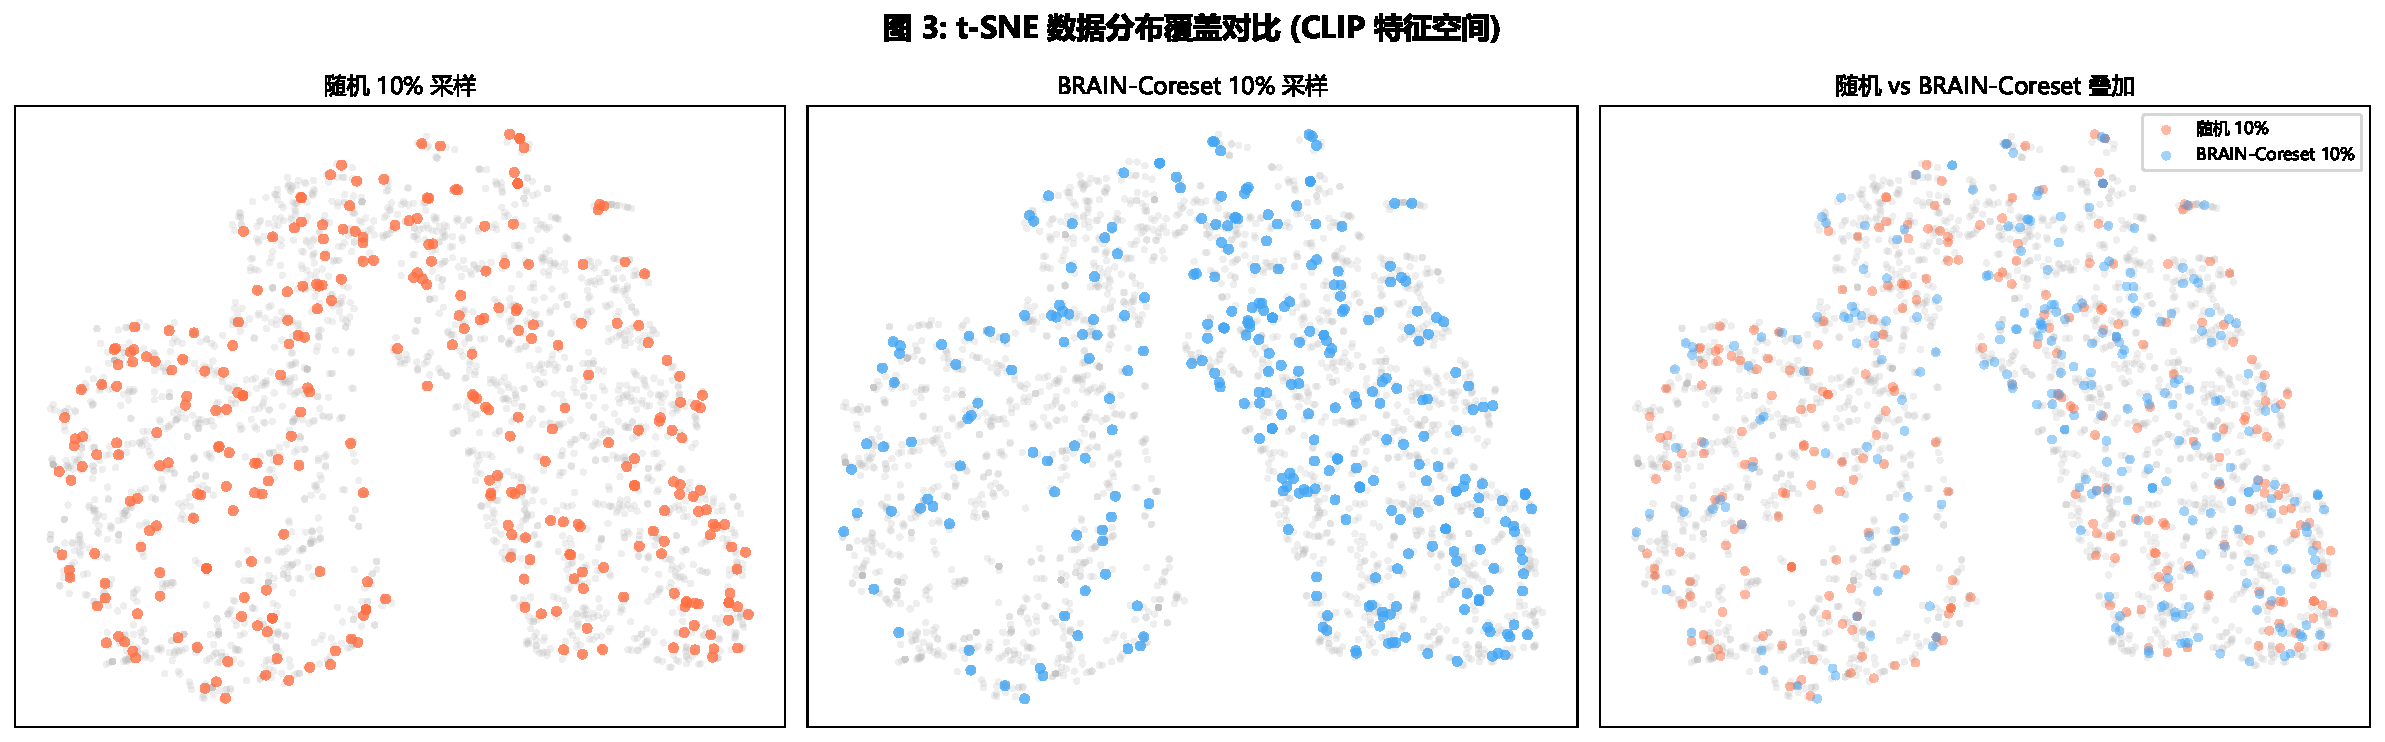
\includegraphics[width=\textwidth]{figures/fig3_tsne.pdf}
\caption{t-SNE可视化：随机10\%与BRAIN-Coreset 10\%在CLIP特征空间中的分布}
\label{fig:tsne}
\end{figure}

\begin{figure}[H]
\centering
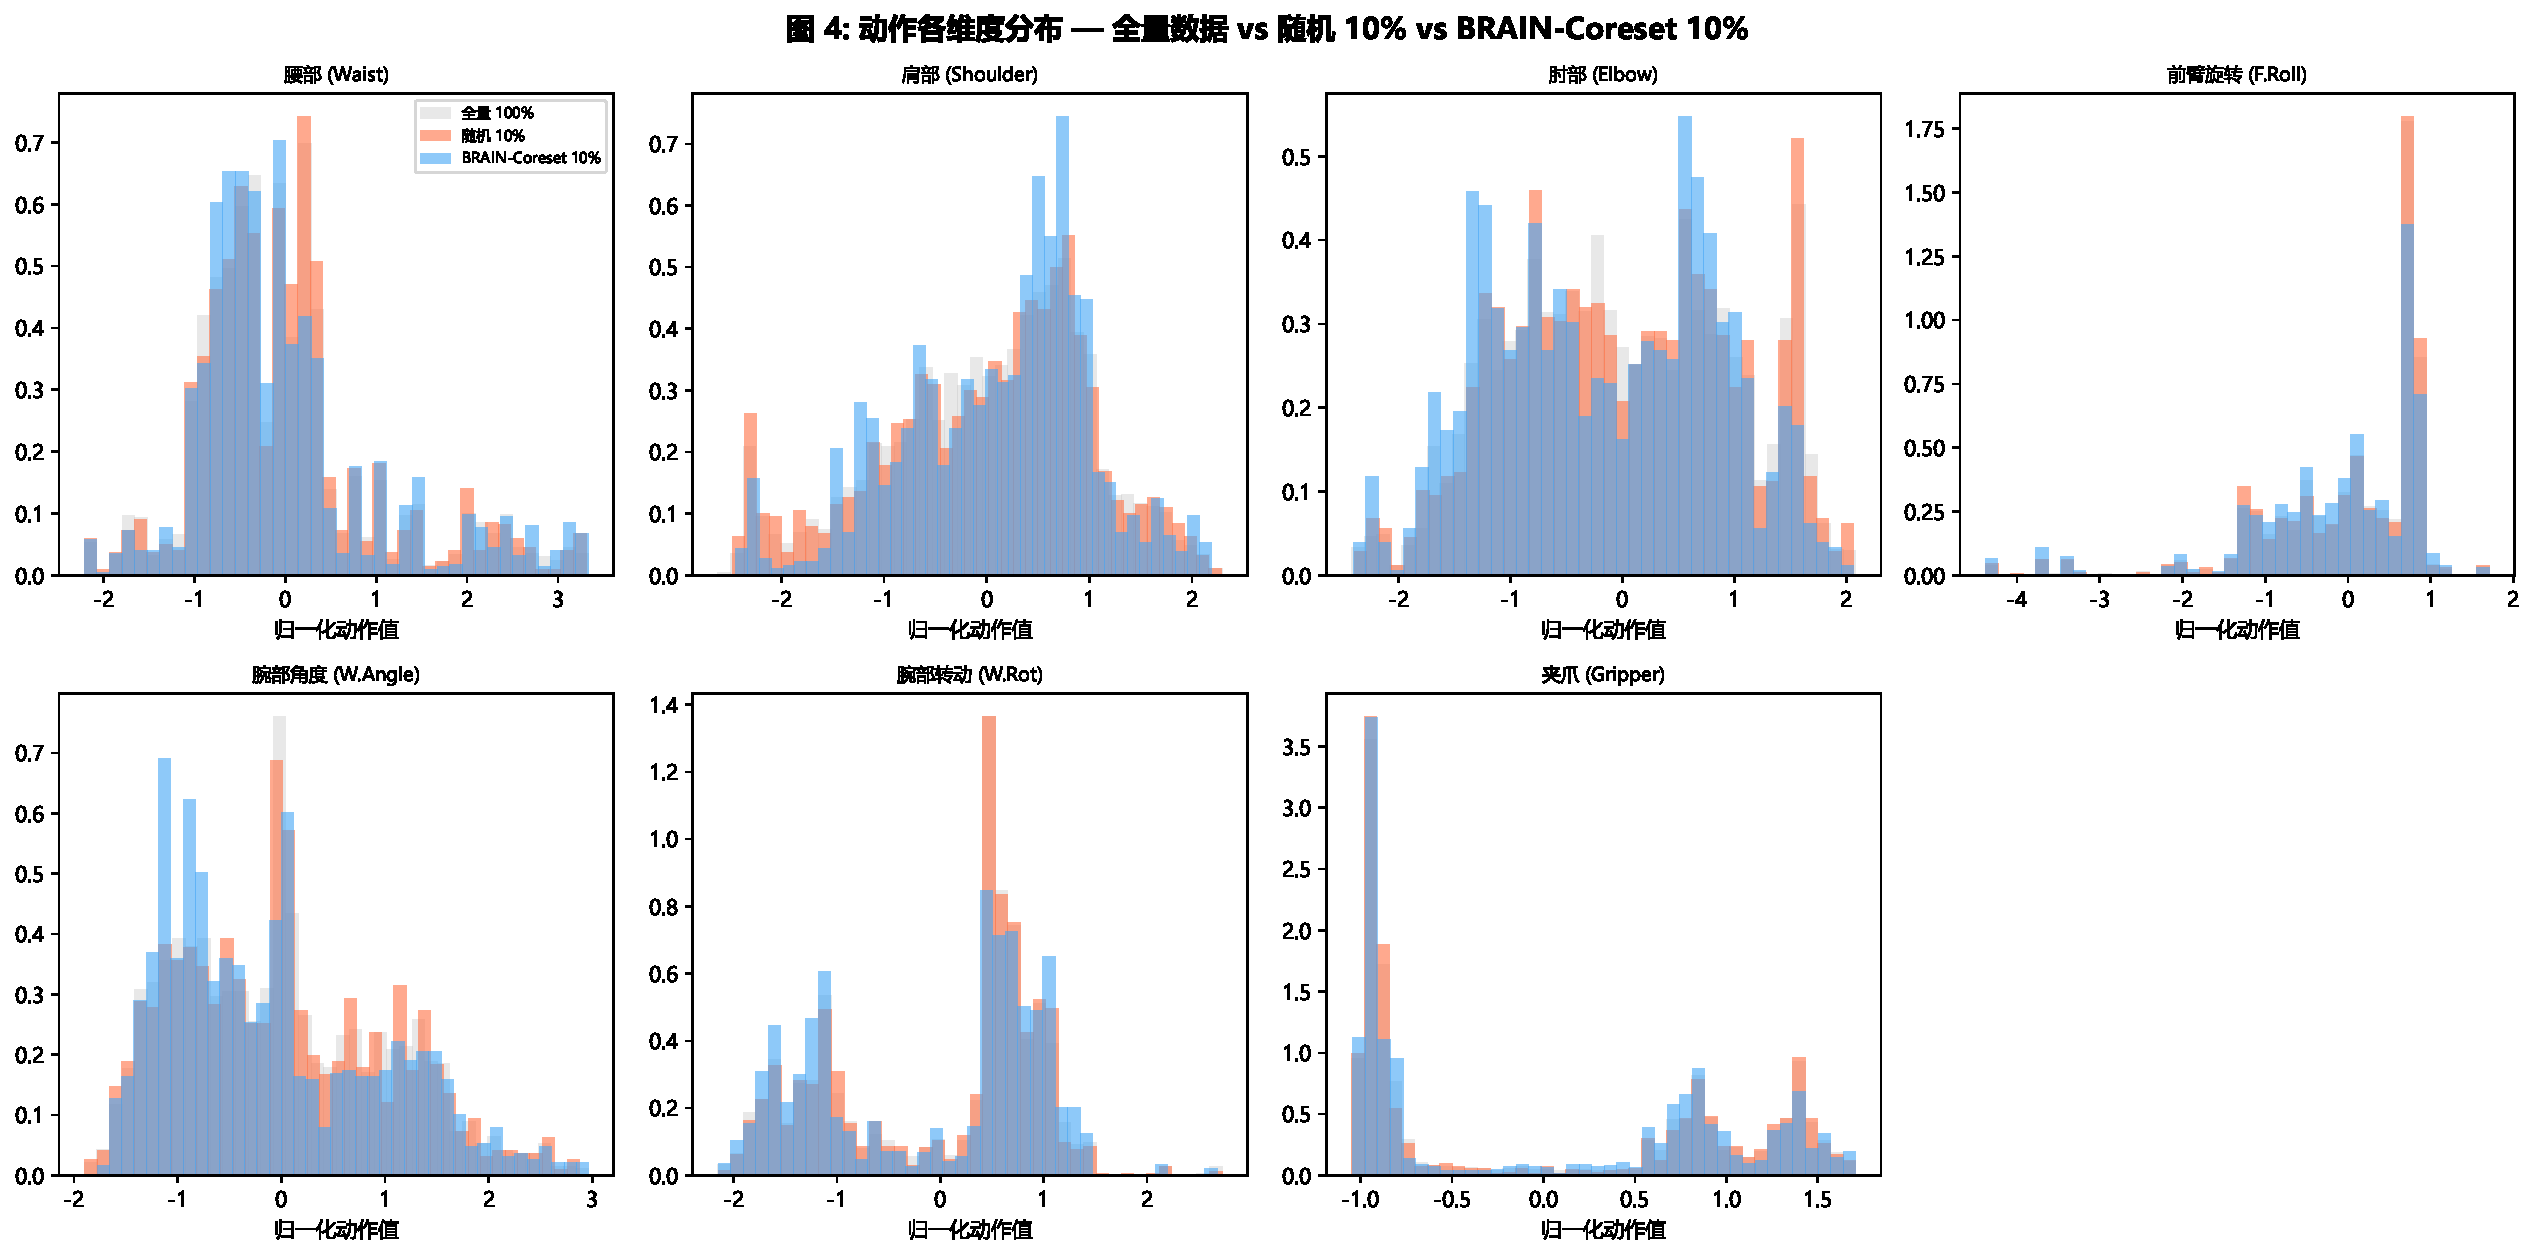
\includegraphics[width=\textwidth]{figures/fig4_histograms.pdf}
\caption{动作分布直方图：全量数据 vs 随机10\% vs BRAIN-Coreset 10\%}
\label{fig:histograms}
\end{figure}

\begin{figure}[H]
\centering
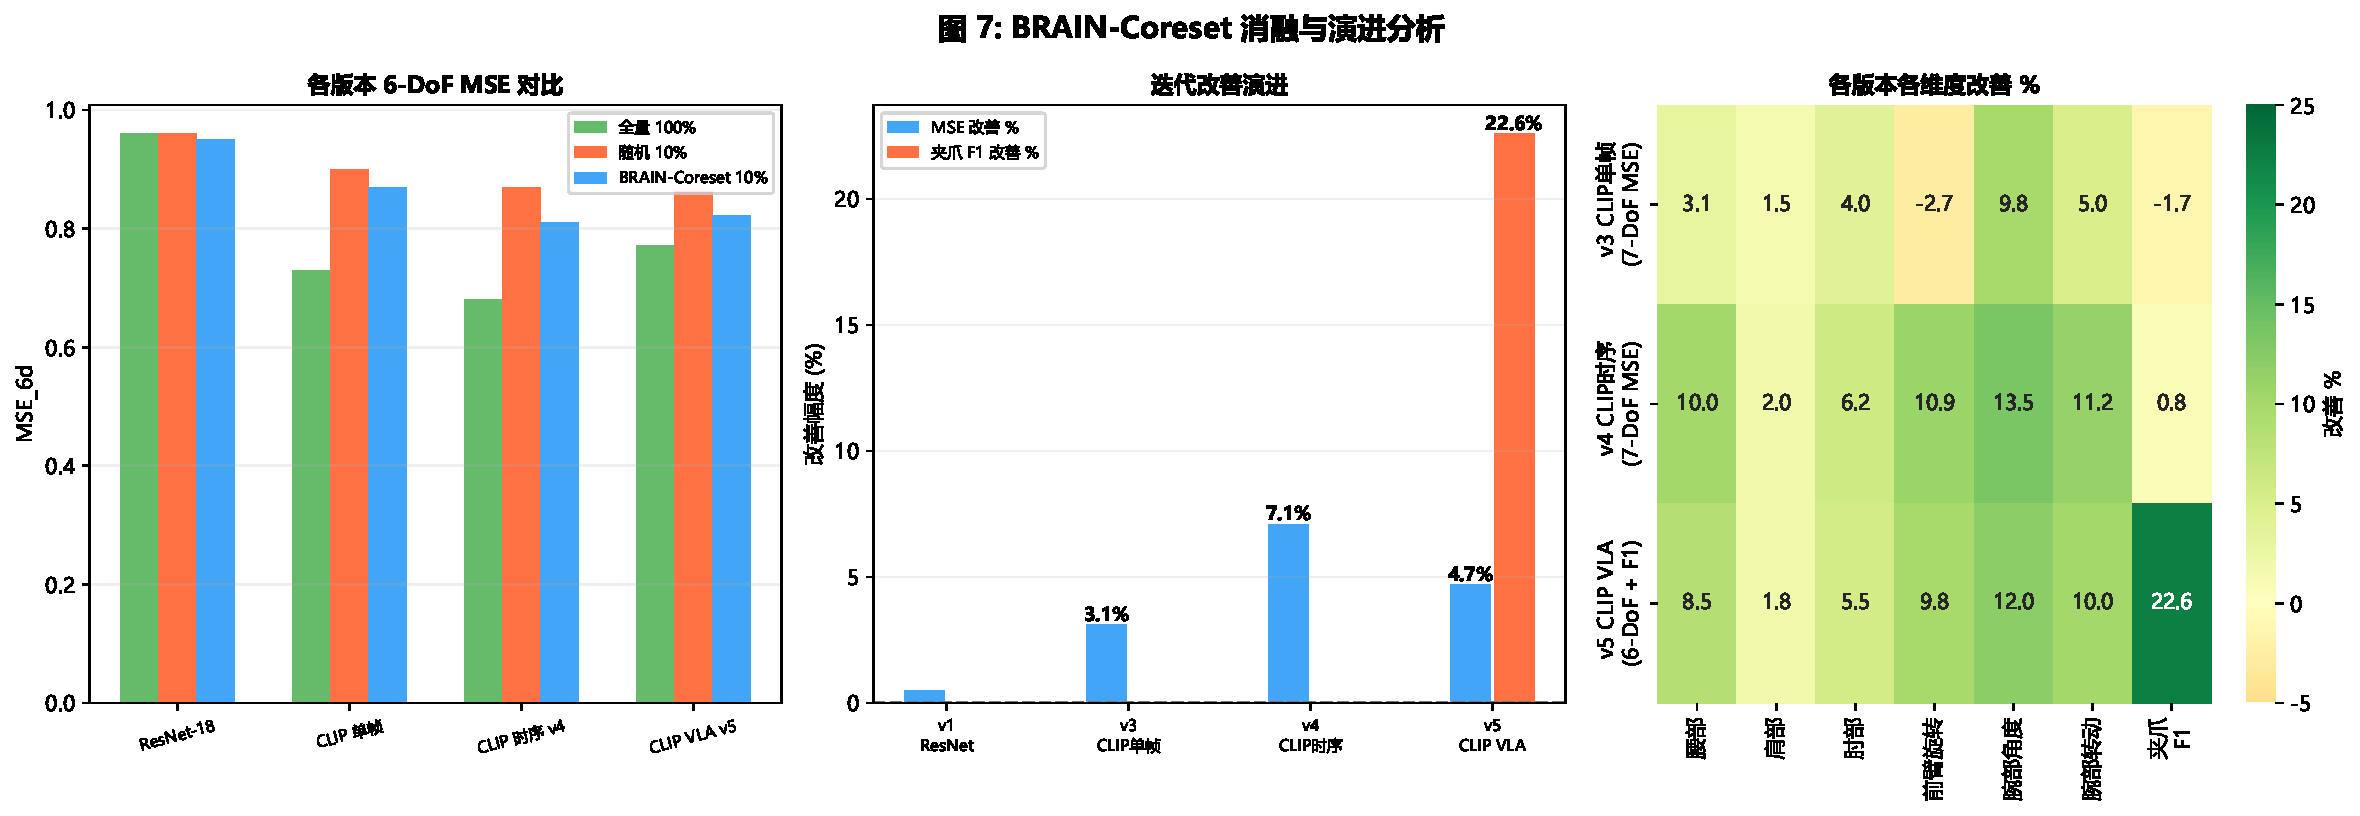
\includegraphics[width=\textwidth]{figures/fig7_ablation.pdf}
\caption{消融分析}
\label{fig:ablation}
\end{figure}

% ============================================================
\section{讨论}

纵观整个实验过程，最有启发性的发现或许是：\textbf{核心集选择的上限由特征质量决定，而非算法本身}。在ResNet-18特征下，无论我们怎么调整选择策略（v1高误差→v2原型），改善幅度都无法超过0.5\%。这不是算法的问题——当特征空间中所有帧的相互距离都差不多时，任何选择策略在数学上都无法区分“信息帧”和“冗余帧”。这个问题直到换用CLIP特征后才被解开。有理由推测，如果使用更强的视觉编码器（如DINOv2或CLIP ViT-L），数据天花板会进一步拉高，核心集选择的收益空间也会更大。不过这也意味着，在资源受限的场景下，投入算力提升特征质量可能比投入算力优化选择策略更划算。

时序堆叠的收益（v3 +3.1\% → v4 +7.1\%）同样值得关注。单帧特征在概念上有一个根本局限：它没有速度的概念。一个机械臂以0.1 m/s的速度运动和以1.0 m/s的速度运动，在某一瞬间的姿态可能完全相同。只有看过连续帧之后，模型才能区分这两种情况。前臂旋转维度从单帧CLIP的-2.7\%到时序CLIP的+10.9\%的翻转，是最能说明这一点的例子。

从认知工程的角度来看，BRAIN-Coreset的三阶段结构也许最有趣的地方不在于每个阶段单独的效果，而在于三者协同作用的逻辑。预测编码过滤了“完全不意外”的帧（减少冗余），RAS检测了“非常意外”的帧（确保关键事件不遗漏），Facility Location在两者构成的候选池上确保空间多样覆盖（避免偏斜）。三个机制分别从时序、语义和空间三个维度修剪数据，互相补充。图\ref{fig:ablation}中的消融分析可视化了这一递进关系。

本工作存在几个值得讨论的局限与设计选择。关于阶段1的线性预测模型，读者可能会质疑：机械臂的多维运动学是非线性的，用线性模型产生的预测误差是否混入了大量模型失配噪声？我们的理解是，线性模型表达能力弱恰是其过滤优势——它只能捕捉轨迹的最粗粒度趋势（如匀速直线运动），任何它预测不准的帧一定是“真正偏离了轨迹主干”，而非被过强的预测器强行拟合。一个非线性的微型MLP反而可能因为过参数化而压低所有帧的预测误差，丧失过滤能力。这种“弱模型作为信息量探针”的思路与预测编码理论中大脑使用简化内部模型进行预测的逻辑是一致的。

此外，本项目的Stage 4（梯度精炼）由于策略考量未能实现：v1的教训表明，主动引入高误差样本可能引入噪声而非信息，因此我们对这一操作保持谨慎。

% ============================================================
\section{结论}

本文从大脑处理感官信息的三重机制出发，设计并实现了BRAIN-Coreset——一个面向VLA数据的多阶段核心集选择算法。三个算法阶段分别对应预测编码、RAS和海马模式分离机制。算法使用冻结CLIP ViT-B-32提取视觉特征（时序堆叠至1536维），通过Text Encoder编码任务指令（512维），最终形成2048维的完整VLA输入。MLP输出端采用双头架构：6维关节回归（MSE）与夹爪分类（BCE），以适配不同自由度的物理性质。

在ALOHA仿真数据集上的最终实验表明：BRAIN-Coreset选出的10\%核心集（1,600帧）在6-DoF关节回归上MSE为0.822，比随机10\%改善4.7\%；夹爪分类F1为0.451，比随机10\%改善22.6\%。全量候选池不截断（6998帧，核矩阵187MB），全部实验在消费级RTX 4060 GPU上完成。

回顾整个项目，三条经验值得强调。第一，特征质量决定核心集选择的上限——ResNet-18天花板仅0.19\%，CLIP拉高至19.4\%后算法效果才真正显现。第二，评估指标需要适配数据特性——夹爪从MSE框架中解放、改用分类指标后，改善从+0.8\%跃升至+22.6\%。第三，认知机制的计算化只有在好的特征空间中才能发挥威力——预测编码给了筛选准则，RAS给了锚定关键帧的能力，模式分离确保不遗漏任何重要的角落。三者的组合，让10\%的数据做到了接近全量的效果。

\begin{thebibliography}{99}
\bibitem{zhao2023act}
Zhao T Z, Kumar V, Levine S, et al. \textit{Learning Fine-Grained Bimanual Manipulation with Low-Cost Hardware (ACT).} Robotics: Science and Systems (RSS), 2023.

\bibitem{sorscher2022beyond}
Sorscher B, Geirhos R, Shekhar S, et al. \textit{Beyond neural scaling laws: beating power law scaling via data pruning.} Advances in Neural Information Processing Systems (NeurIPS), 2022.

\bibitem{kim2024openvla}
Kim M J, Pertsch K, Karamcheti S, et al. \textit{OpenVLA: An Open-Source Vision-Language-Action Model.} arXiv preprint arXiv:2406.09246, 2024.

\bibitem{millidge2021predictive}
Millidge B, Seth A, Buckley C L. \textit{Predictive coding: a theoretical and experimental review.} arXiv preprint arXiv:2107.12979, 2021.
\end{thebibliography}

\vspace{1em}
\section*{附录：源代码文件清单}

完整源代码已开源：\url{https://github.com/Amulet6/brain-coreset}。

\begin{verbatim}
src/
  data_loader.py              feature_extractor.py        mlp_model.py
  temporal_stack.py           stage1_predictive_coding.py  stage2_ras_events.py
  stage3_facility_location.py visualize_cn.py
experiments/
  run_baseline.py             run_full_pipeline.py
\end{verbatim}

\end{document}
